%%%%%%%%%%%%%%%%%%%%%%%%%%%%%%%%%%%%%%%%%%%%%%%
% BEGIN Cirkelbeweging
%%%%%%%%%%%%%%%%%%%%%%%%%%%%%%%%%%%%%%%%%%%%%%%
\chapter{Cirkelbeweging}

Dit hoofdstuk behandelt beweging in poolcoordinaten en in het bijzonder de eenparige
cirkelbeweging. Belangrijke begrippen als centripetaalkracht worden behandeld in dit
hoofdstuk.

Stof uit Giancoli:
\begin{itemize}
\item Hoofdstuk 5.2-5.5
\end{itemize}


\section{Beweging in poolcoordinaten}

Waarschuwing: deze paragraaf behandelt poolcoordinaten in het algemeen en is behoorlijk pittig. 
Voor de liefhebbers en fijnproevers dus, want we zullen bijna altijd het speciale geval van eenparige
cirkelbeweging tegenkomen in onze opgaven. Eenparige cirkelbeweging komt in de volgende paragraaf
aan bod.

\begin{center}
\line(1,0){250}
\end{center}

Als je te maken krijgt met een centrale kracht blijkt het handig te zijn om niet in cartesische 
coordinaten te werken, maar bijvoorbeeld in poolcoordinaten. 
 \begin{figure}[htbp]
\begin{center}
  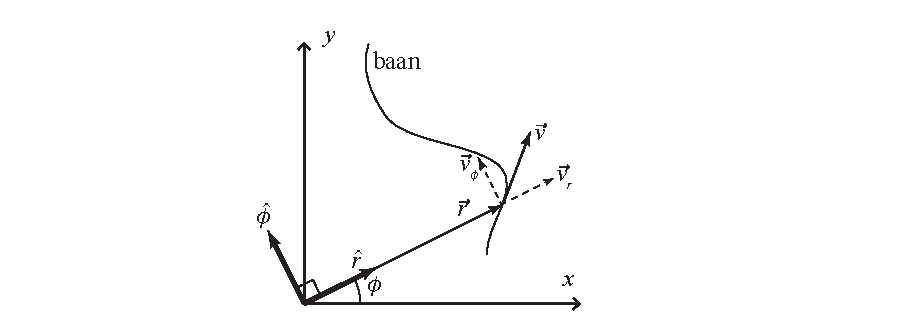
\epsfig{file=PoolCoordinaten.pdf, width=\textwidth}
\caption{{\it Positie en snelheid in poolcoordinaten.}}
\label{fig:pool}
\end{center}
\end{figure} 
Met poolcoordinaten kan je 
een positie in een 2-D vlak uitdrukken in termen van een afstand tot de oorsprong van het 
coordinatensysteem, $r$, en een hoek $\phi$, zoals aangegeven in Fig.~\ref{fig:pool}.  
\begin{equation}
\vec{r} = r \hat{r}
\end{equation}
met:
\begin{equation}
\hat{r} = (\cos\phi,\,\sin\phi)
\end{equation}
Deze laatste vector is een eenheidsvector ({\it laat zien}), die gericht staat in de radiele
richting ({\it laat zien}).  Naast een eenheidsvector in de radiele richting is het ook 
mogelijk een eenheidsvector, $\hat{\phi}$, te construeren in de azimuthale richting:
\begin{equation}
\hat{\phi} = (-\sin\phi,\,\cos\phi)
\end{equation}
Deze vector staat loodrecht op $\hat{r}$ en heeft ook lengte 1. Het blijkt dat je beweging
in het 2-D vlak met behulp van $r$, $\phi$, $\hat{r}$ en $\hat{\phi}$ volledig kan 
karakteriseren net zoals je dat kan met cartesische coordinaten. In eerste instantie kan
dit misschien iets lastiger lijken, omdat je eenheidsvectoren afhangen van de coordinaat $\phi$,
terwijl ze in cartesische coordinaten mooi constant waren. 

\begin{center}
\line(1,0){250}
\end{center}
\begin{voorbeeld} 
(i) Bewijs dat $\hat{r}$ en $\hat{\phi}$ loodrecht op elkaar staan. (ii) Bewijs dat $\hat{\phi}$ lengte~1
heeft.

{\bf Oplossing: }{\it (i) Voor het inproduct tussen twee vectoren $\vec{A}$ en $\vec{B}$ in 2-D geldt:
\begin{equation}
\vec{A}\cdot\vec{B} = A_x\,B_x+A_y\,B_y = |\vec{A}||\vec{B}|\cos\alpha
\end{equation}
Met $\alpha$ de hoek tussen de twee vectoren. Dus voor $\hat{r}$ en $\hat{\phi}$:
\begin{equation}
\hat{r}\cdot\hat{\phi} = \cos\phi\,(-\sin\phi)+\sin\phi \,\cos\phi = 0
\end{equation}
Dit impliceert dat $\alpha=\pi/2$ en dus staan de twee vectoren loodrecht op elkaar.
(ii) De lengte van een vector, $L$, is uit te rekenen door:
\begin{eqnarray}
L & = & \sqrt{\hat{\phi}\cdot\hat{\phi}} \\
& = & \sqrt{(-\sin\phi)^2+(\cos\phi)^2} \\
& = & 1
\end{eqnarray}
Q.E.D.
}
\end{voorbeeld}
\begin{center}
\line(1,0){250}
\end{center}

De snelheid van een object is zoals gewoonlijk weer gegeven door
te tijdsafgeleide te nemen van de positie. Maar nu moet je goed uitkijken, want
de tijdsafgeleide van de eenheidsvector $\hat{r}\neq\vec{0}$! Laten we eens kijken
hoe de snelheid eruit ziet:
\begin{eqnarray}
\vec{v} &=& \frac{d\vec{r}}{dt} \\
& = & \frac{dr}{dt} \hat{r} + r \frac{d\hat{r}}{dt}
\end{eqnarray} 
Laten we de tijdsafgeleide van de radiele eenheidsvector eens bekijken:
\begin{eqnarray}
\frac{d\hat{r}}{dt} & = & \frac{d}{dt}(\cos\phi,\,\sin\phi) \\
& = & \frac{d\phi}{dt}\,(-\sin\phi,\,\cos\phi) \\
& = & \frac{d\phi}{dt}\,\hat{\phi}
\end{eqnarray}
Dat is natuurlijk mooi: de tijdsafgeleide van de radiele eenheidsvector geeft
je een vector in de $\phi$ richting. We kunnen nu de snelheid schrijven als:
\begin{equation}\label{eq:vpool}
\vec{v} = \frac{dr}{dt} \hat{r} + r\frac{d\phi}{dt} \hat{\phi} = \vec{v}_{r}+\vec{v}_{\phi}
\end{equation}
De snelheid bestaat dus uit een component langs de baan van het object en
een component loodrecht daarop, in de radiele richting. Een uitdrukking als
hierboven mag je ook niet echt verbazen, want het zou natuurlijk vreemd zijn
als er een snelheid zou worden gevonden zonder $\hat{\phi}$ component. 
Daarnaast kan je zien dat de tangentiele of $\hat{\phi}$ component van de
snelheid afhangt  van de hoeksnelheid $\omega\equiv d\phi / dt$ maal
de afstand tot de oorsprong. Ook niet zo vreemd, want een kleine hoeksnelheid
met bijvoorbeeld een grote afstand kan leiden tot een grote baansnelheid, en
vice-versa.

Tenslotte kunnen we kijken hoe de versnelling van een object eruit ziet in 
poolcoordinaten. Daarvoor moeten we de tijdsafgeleide nemen van de snelheid
en dat is even stug differentieerwerk:
\begin{eqnarray}
\vec{a} & = & \frac{d\vec{v}}{dt} \\
 & = & \frac{d^2r}{dt^2}\hat{r}  + \frac{dr}{dt}\,\frac{d\hat{r}}{dt} + \frac{d}{dt}\left(r\frac{d\phi}{dt}\right)\hat{\phi} + r\frac{d\phi}{dt}\frac{d\hat{\phi}}{dt} \\ 
 & = & \left\{\frac{d^2r}{dt^2}-r\left(\frac{d\phi}{dt}\right)^2\right\}\hat{r}+\left\{2\frac{dr}{dt}\frac{d\phi}{dt}+r\frac{d^2\phi}{dt^2}\right\}\hat{\phi}\label{eq:apool} \\
 & = & \vec{a}_{r}+\vec{a}_{\phi}
 \end{eqnarray}
 In de iedere stap is gebruik gemaakt van de productregel voor differentieren, en in de laatste stap is de 
 afgeleide van $\hat{\phi}$ uitgerekend:
 \begin{equation}
 \frac{d\hat{\phi}}{dt} = -\frac{d\phi}{dt}\hat{r}
 \end{equation}
Deze vergelijking ziet er behoorlijk intimiderend uit en bevat een behoorlijke hoeveelheid 
afgeleiden en dubbele afgeleiden. En de vraag is waarom zou je nou een dergelijke vergelijking 
willen gebruiken. 

\begin{center}
\line(1,0){250}
\end{center}
\begin{voorbeeld} 
Een object beweegt over een cirkel met constante straal $r(t)=R$. De hoek $\phi(t)$ wordt gegeven door
$\phi(t) = a_0 +a_1\,t +\frac{1}{2} \, a_2\,t^2$. Bereken (i) de snelheid $\vec{v}(t)$ en (ii) de versnelling $\vec{a}(t)$.

{\bf Oplossing: }{\it (i) We hoeven alleen maar onze vergelijking voor $\phi(t)$ in te vullen in de
vergelijking voor de snelheid~\ref{eq:vpool} en ons te bedenken dat $dR/dt=0$:
\begin{eqnarray}
\vec{v} & = & \frac{dR}{dt}\hat{r} + R\frac{d\phi}{dt}\hat{\phi} \\
& = & R\left(a_1 + a_2\,t\right)\hat{\phi}
\end{eqnarray}
De snelheid heeft dus alleen een $\hat{\phi}$ component, wat je natuurlijk ook verwacht voor een baan
met constante straal. (ii) De versnelling wordt gegeven door vgl.~\ref{eq:apool}. Invullen levert:
\begin{eqnarray}
\vec{a} & = & -R\left(a_1+a_2\,t\right)^2\,\hat{r} + R\,a_2\,\hat{\phi}
\end{eqnarray}
De versnelling heeft dus wel degelijk een $\hat{r}$ component, ondanks dat de straal van de baan constant 
is! (Ga zelf na wat de eenheden van de constanten $a_0$, $a_1$ en $a_2$ moeten zijn, en controleer dat de
dimensie van het antwoord klopt.
}
\end{voorbeeld}
\begin{center}
\line(1,0){250}
\end{center}
 

\section{Eenparige cirkelbeweging}

De vergelijkingen voor beweging in poolcoordinaten kunnen uitstekend worden toegepast 
in het geval van eenparige cirkelbeweging zoals getekend in Fig.~\ref{fig:cirkel}. 
 \begin{figure}[htbp]
\begin{center}
  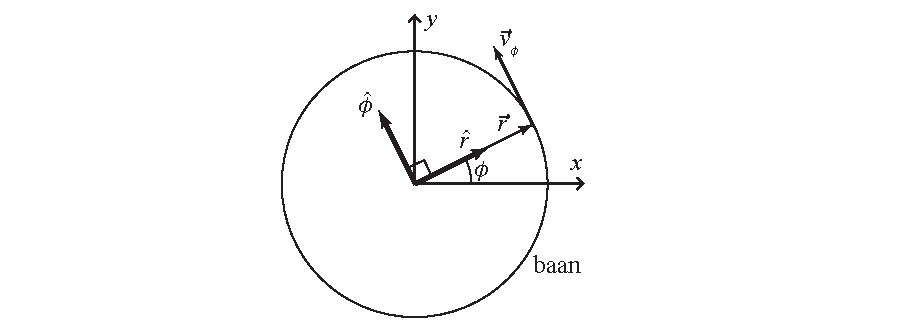
\epsfig{file=EenparigeCirkel.pdf, width=\textwidth}
\caption{{\it Eenparige cirkelbeweging.}}
\label{fig:cirkel}
\end{center}
\end{figure} 
Bij eenparige 
cirkelbeweging is er sprake van een beweging op een cirkel met constante straal en een
constante hoeksnelheid. Dus:
\begin{eqnarray}
\frac{dr}{dt} & = & 0\\
\frac{d^2r}{dt^2} & = & 0 \\
\frac{d\phi}{dt} &= & \omega = \mbox{constant} \\
\frac{d^2\phi}{dt^2} & = & 0
\end{eqnarray}
Het gevolg is dat de vergelijkingen voor snelheid en versnelling nu in poolcoordinaten er 
een stuk eenvoudiger uitzien dan in cartesische coordinaten. Voor de snelheid zoals in
vgl.~\ref{eq:vpool} geldt nu:
\begin{eqnarray}\label{eq:vpoolcir}
\vec{v} & =&  \vec{v}_{\phi} \\
             & =& \omega\,R\,\hat{\phi}
\end{eqnarray}
Hierin is de constante straal van de baan, $R$, en de hoeksnelheid $\omega$ is weer 
$d\phi / dt$. Ook de hoeksnelheid is nu constant.

De vergelijking  voor de versnelling in poolcoordinaten~\ref{eq:apool} reduceert nu tot:
\begin{eqnarray}\label{eq:apoolcir}
\vec{a} & = & -\omega^2\,R\,\hat{r}
\end{eqnarray}
En dit is een stuk eenvoudiger dan de versnelling in cartesische coordinaten. Bovendien
leer je direct uit deze vergelijking dat er een versnelling in de radiele richting nodig is om een
eenparige cirkelbeweging te laten plaatsvinden. De richting van deze versnelling is naar
het centrum van de cirkel gericht en heet de {\emph centripetale} ofwel middelpuntzoekende
versnelling. Vaak wordt er gesproken over een centrifugale of middelpuntvliedende versnelling,
maar meestal zijn het geen natuurkundigen die een dergelijke discussie voeren. Er bestaat
namelijk niet zoiets als een centrifugale versnelling: als de centripetale versnelling er niet
zou zijn dan beweeg je gewoon weer met een constante snelheid. Wat verder opmerkelijk is 
aan de eenparige cirkelbeweging, is dat een object continue een versnelling ondervindt, 
terwijl de grootte van de snelheid niet verandert.

Tenslotte kan je vgl.~\ref{eq:apoolcir} met gebruik van de vergelijking voor de snelheid~\ref{eq:vpoolcir}
herschrijven tot:
\begin{equation}
\vec{a} = -\frac{|\vec{v}|^2}{R}\hat{r}
\end{equation}
De bijbehorende centripetale kracht, $\vec{F}_C$ nodig om een object met massa $m$ in een baan met straal $R$
te houden is nu natuurlijk direct te schrijven schrijven als:
\begin{equation}\label{eq:fc_cirkel}
\vec{F}_C = -\frac{m\,|\vec{v}|^2}{R}\hat{r}
\end{equation}
De centripetale kracht is dus evenredig met $|\vec{v}|^2$ en dat betekent dat de kracht snel 
groter wordt als je snel door een bocht wil. Eveneens wordt de kracht veel groter als je een
kleine draaicirkel kiest.

\begin{center}
\line(1,0){250}
\end{center}
\begin{voorbeeld} 
Een slinger met lengte $l$ zoals getekend in Fig.~\ref{fig:cirkelvoorbeeld}~a) draait met constante
snelheid rondjes (\emph{let op: de grootte van de snelheid is constant, de richting verandert}). Bereken 
de hoek $\theta$.
 \begin{figure}[htbp]
\begin{center}
  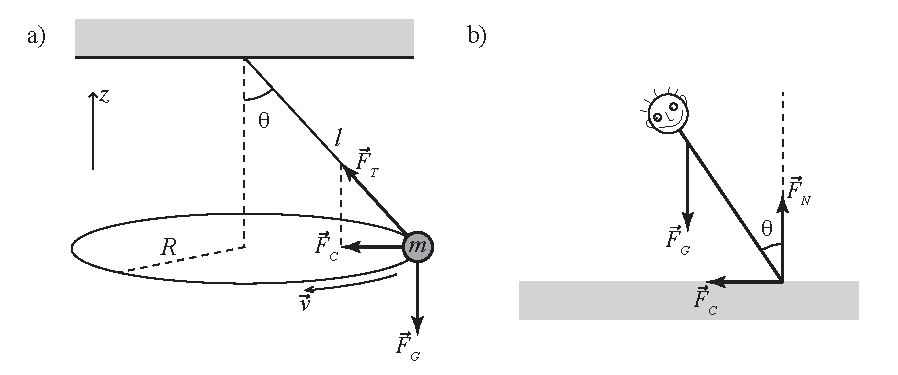
\epsfig{file=CentripetaalVoorbeeld.pdf, width=\textwidth}
\caption{{\it a) Ronddraaiende slinger. b) Colijn in de bocht.}}
\label{fig:cirkelvoorbeeld}
\end{center}
\end{figure} 

{\bf Oplossing: }{\it De eerste stap voor de oplossing van dit probleem is het maken van een tekening met alle krachten
op de massa $m$ zoals in Fig.~\ref{fig:cirkelvoorbeeld}~a) staan aangegeven.  Naast de $\hat{r}$ en $\hat{\phi}$ 
coordinaat kiezen we ook een $z$-as zoals getekend. De $z$ component van de spankracht, $\vec{F}_T$ in de slinger 
is even groot als de zwaartekracht op de massa, maar tegengesteld van richting. De massa beweegt immers met 
constante snelheid en hangt dus op constante $z$. Dus;
\begin{equation}
m\,g = |\vec{F}_T|_z = |\vec{F}_T|\cos\theta
\end{equation}
De radiele component van de spankracht zorgt levert de centripetale versnelling om de massa in de bocht te houden. De
straal $R$ van de baan is gegeven door $R=l \sin\theta$. We kunnen schrijven:
\begin{eqnarray}
|\vec{F}_C| & = & |\vec{F}_T|_r\\
\frac{m|\vec{v}|^2}{R} & = & |\vec{F}_T|\sin\theta \\
\frac{m|\vec{v}|^2}{l\sin\theta} & = & |\vec{F}_T|\sin\theta
\end{eqnarray}
Nu kunnen we listig de laatste vergelijking delen door de vorige. Op die manier raken we de spankracht 
kwijt uit onze vergelijking en krijgen we de volgende uitdrukking:
\begin{eqnarray}
\tan\theta & = & \frac{|\vec{v}|^2}{l\,\sin\theta\,g} \\
& \Downarrow & \\
\frac{\sin^2\theta}{\cos\theta} & = & \frac{|\vec{v}|^2}{l\,g}
\end{eqnarray}
De uitwijking hangt dus alleen maar af van de snelheid, de lengte van de slinger en $g$. De massa speelt geen rol voor
de uitwijking, maar uiteraard wel voor de spankracht in het touw. Reken die maar eens uit.
}
\end{voorbeeld}
\begin{center}
\line(1,0){250}
\end{center}
\begin{voorbeeld} 
Docent Colijn gaat door de bocht met snelheid $\vec{v}$ ($|\vec{v}|$ is constant) op een oppervlak met statische wrijving, 
gekarakteriseerd door wrijvingscoefficient $\mu_s$ zoals in Fig.~\ref{fig:cirkelvoorbeeld}~b). 
(i) Druk de hoek $\theta$ uit in bekende grootheden. (ii) Wat is de minimale straal $R$ van de bocht, zonder dat Colijn uitglijdt?  

{\bf Oplossing:}{\it (i) Teken alle krachten op Colijn. Uit de tekening blijkt dat de hoek $\theta$ wordt gegeven door:
\begin{eqnarray}
\tan\theta & = & \frac{|\vec{F}_C|}{|\vec{F}_N|} \\
& = & \frac{|\vec{v}|^2}{R\,g}
\end{eqnarray}
Weer onafhankelijk van de massa. Tweewielers die met dezelfde snelheid door de bocht gaan, maken altijd exact dezelfde
hoek met het wegdek. De wrijvingskracht zorgt ervoor dat hier de centripetaalkracht wordt geleverd: als je dus maar snel genoeg 
door de bocht gaat zal je uiteindelijk uitglijden. Vaak wordt een wegdek onder een zodanige hoek aangelegd dat 
de centripetaal versnelling bij een vooraf gekozen snelheid volledig wordt geleverd door de normaalkracht. Zulke bochten
zijn comfortabel, ook voor passagiers van een auto, omdat ze niet zijwaarts worden versneld. (ii) Deze discussie 
brengt ons meteen bij de tweede vraag. De minimale straal van de bocht voor een gegeven snelheid $v$ wordt gevonden 
door de centripetale kracht gelijk te stellen aan de maximale wrijvingskracht:
\begin{eqnarray}
\frac{m|\vec{v}|^2}{R} & = & \mu_s \,m\,g \\
& \Downarrow& \\
R_{min} & = & \frac{|\vec{v}|^2}{\mu_s \,g}
\end{eqnarray}
De minimale straal, $R_{min}$, neemt dus kwadratische toe met de snelheid. daarnaast zie je dat als er weinig 
wrijving is de minimale straal ook toeneemt. Als de wrijving erg klein is - denk aan het lopen op een net gepoetste 
ijsbaan - zie je dat het erg moeilijk wordt om kleine rondjes te draaien.
}
\end{voorbeeld}
\begin{center}
\line(1,0){250}
\end{center}

% \section{Centrale krachten}

\section{Wat moet ik weten en kunnen?}

Na bestuderen van dit hoofdstuk moet je weten:
\begin{itemize}
\item Hoe positie, snelheid en versnelling eruit zien in poolcoordinaten.
\item Hoe je een cirkelbeweging beschrijft.
\item Wat centripetaalkracht is.
\end{itemize}
En je moet kunnen:
\begin{itemize}
\item Rekenen met poolcoordinaten.
\item Rekenen met centripetaalkrachten.
\end{itemize}

\section{Opgaven}

\begin{enumerate}
\item Selectie Giancoli hoofdstuk 5:  46, 47, 54, 62, 64, 80, 87, 92, 93, 100, 101
\item Op een schijf die draait met constante hoeksnelheid $\omega$ bevindt zich 
een karretje met massa $m$ zoals in Fig.~\ref{fig:BalInBuis}. 
 \begin{figure}[htbp]
\begin{center}
  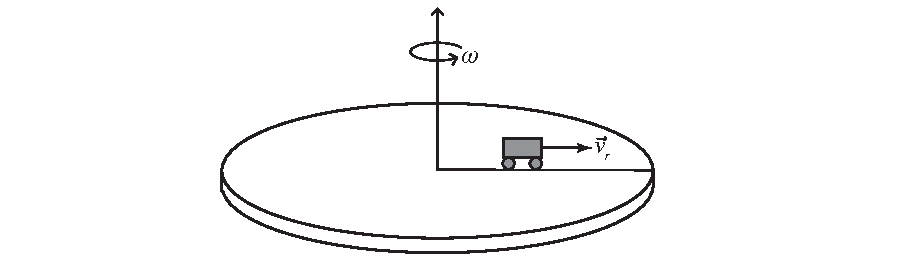
\epsfig{file=BalInBuis.pdf, width=\textwidth}
\caption{{\it Een karretje op een draaiende schijf.}}
\label{fig:BalInBuis}
\end{center}
\end{figure} 
In de radiele richting 
kan het  karretje vrij bewegen, terwijl deze in de $\phi$ richting meedraait met de schijf.
Stel een vergelijking op voor de radiele snelheid als functie van de tijd. Kan je deze
vergelijking oplossen?
\item Waarom spreken zoveel mensen van centrifugaalkrachten? Kan je dit begrijpen? 
Leg uit.
\item Een systeem zoals getekend in Fig.~\ref{fig:flyball} draait rond met hoeksnelheid
$\omega$. Massa $M$ kan vrij glijden over de draaias van het systeem. Bereken
hoek $\theta$.
 \begin{figure}[htbp]
\begin{center}
  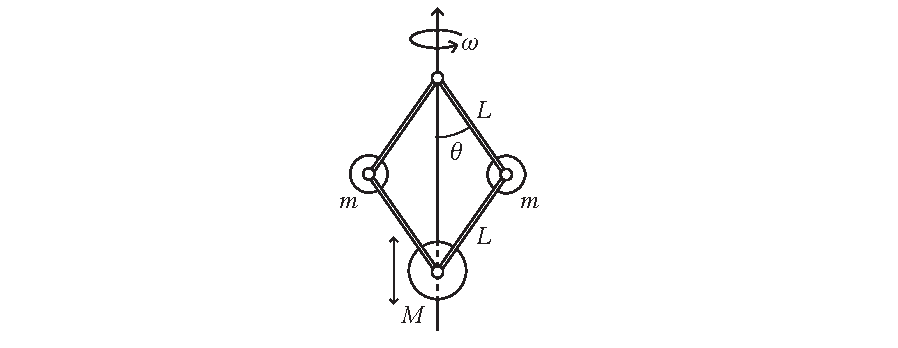
\epsfig{file=FlyballGovernor.pdf, width=\textwidth}
\caption{{\it Glijdende en draaiende massa's.}}
\label{fig:flyball}
\end{center}
\end{figure} 

\end{enumerate}


